\section{Hablaremos del PIB}
\emph{\textbf{Definición de ``Economía de escala'':} la productividad marginal es la productividad de \textbf{un} factor cuando el otro está fijo, relacionamos con la economía de escala, cómo aumenta la producción total cuando aumentan  \textbf{todos los factores}, concepto de deseconomía de escala es cuando a pesar de aumentar la producción total decrece.El PIB nominal, bienes y servicios producidos en un año multiplicados por su precio, El PIB real, bienes y servicios producidos en un año multiplicados por su precio del año anterior}. \newline 
\begin{enumerate}
    \item El tema de PIB, \textbf{Nos preguntamos:} ¿POR QUÉ HAY PAÍSES POBRES Y RICOS? \textbf{Nos preguntamos:} ¿por qué no hay riqueza en todos los países?
    \item \emph{\textbf{Ejemplo:}en China no hay hambre, pero hay una diferencia entre vivir en Shangai y vivir en Tibet, hay países más ricos que otros El Producto Interno Bruto permite medir numéricamente la riqueza de un país.}
    \item \emph{\textbf{Definición de ``PIB":} la suma de todos los bienes producidos que son finales, se utiliza como proxy de riqueza; producción de bienes finales en un año dividido el número de personas.} \textbf{Nos preguntamos:} ¿Cómo se calcula la desigualdad en el PIB? \emph{\textbf{La respuesta a esta esta pregunta es: }el índice de Gini, la curva de Lorent, presentado a continuación.}
    \begin{figure}[htbp]
        \centering
        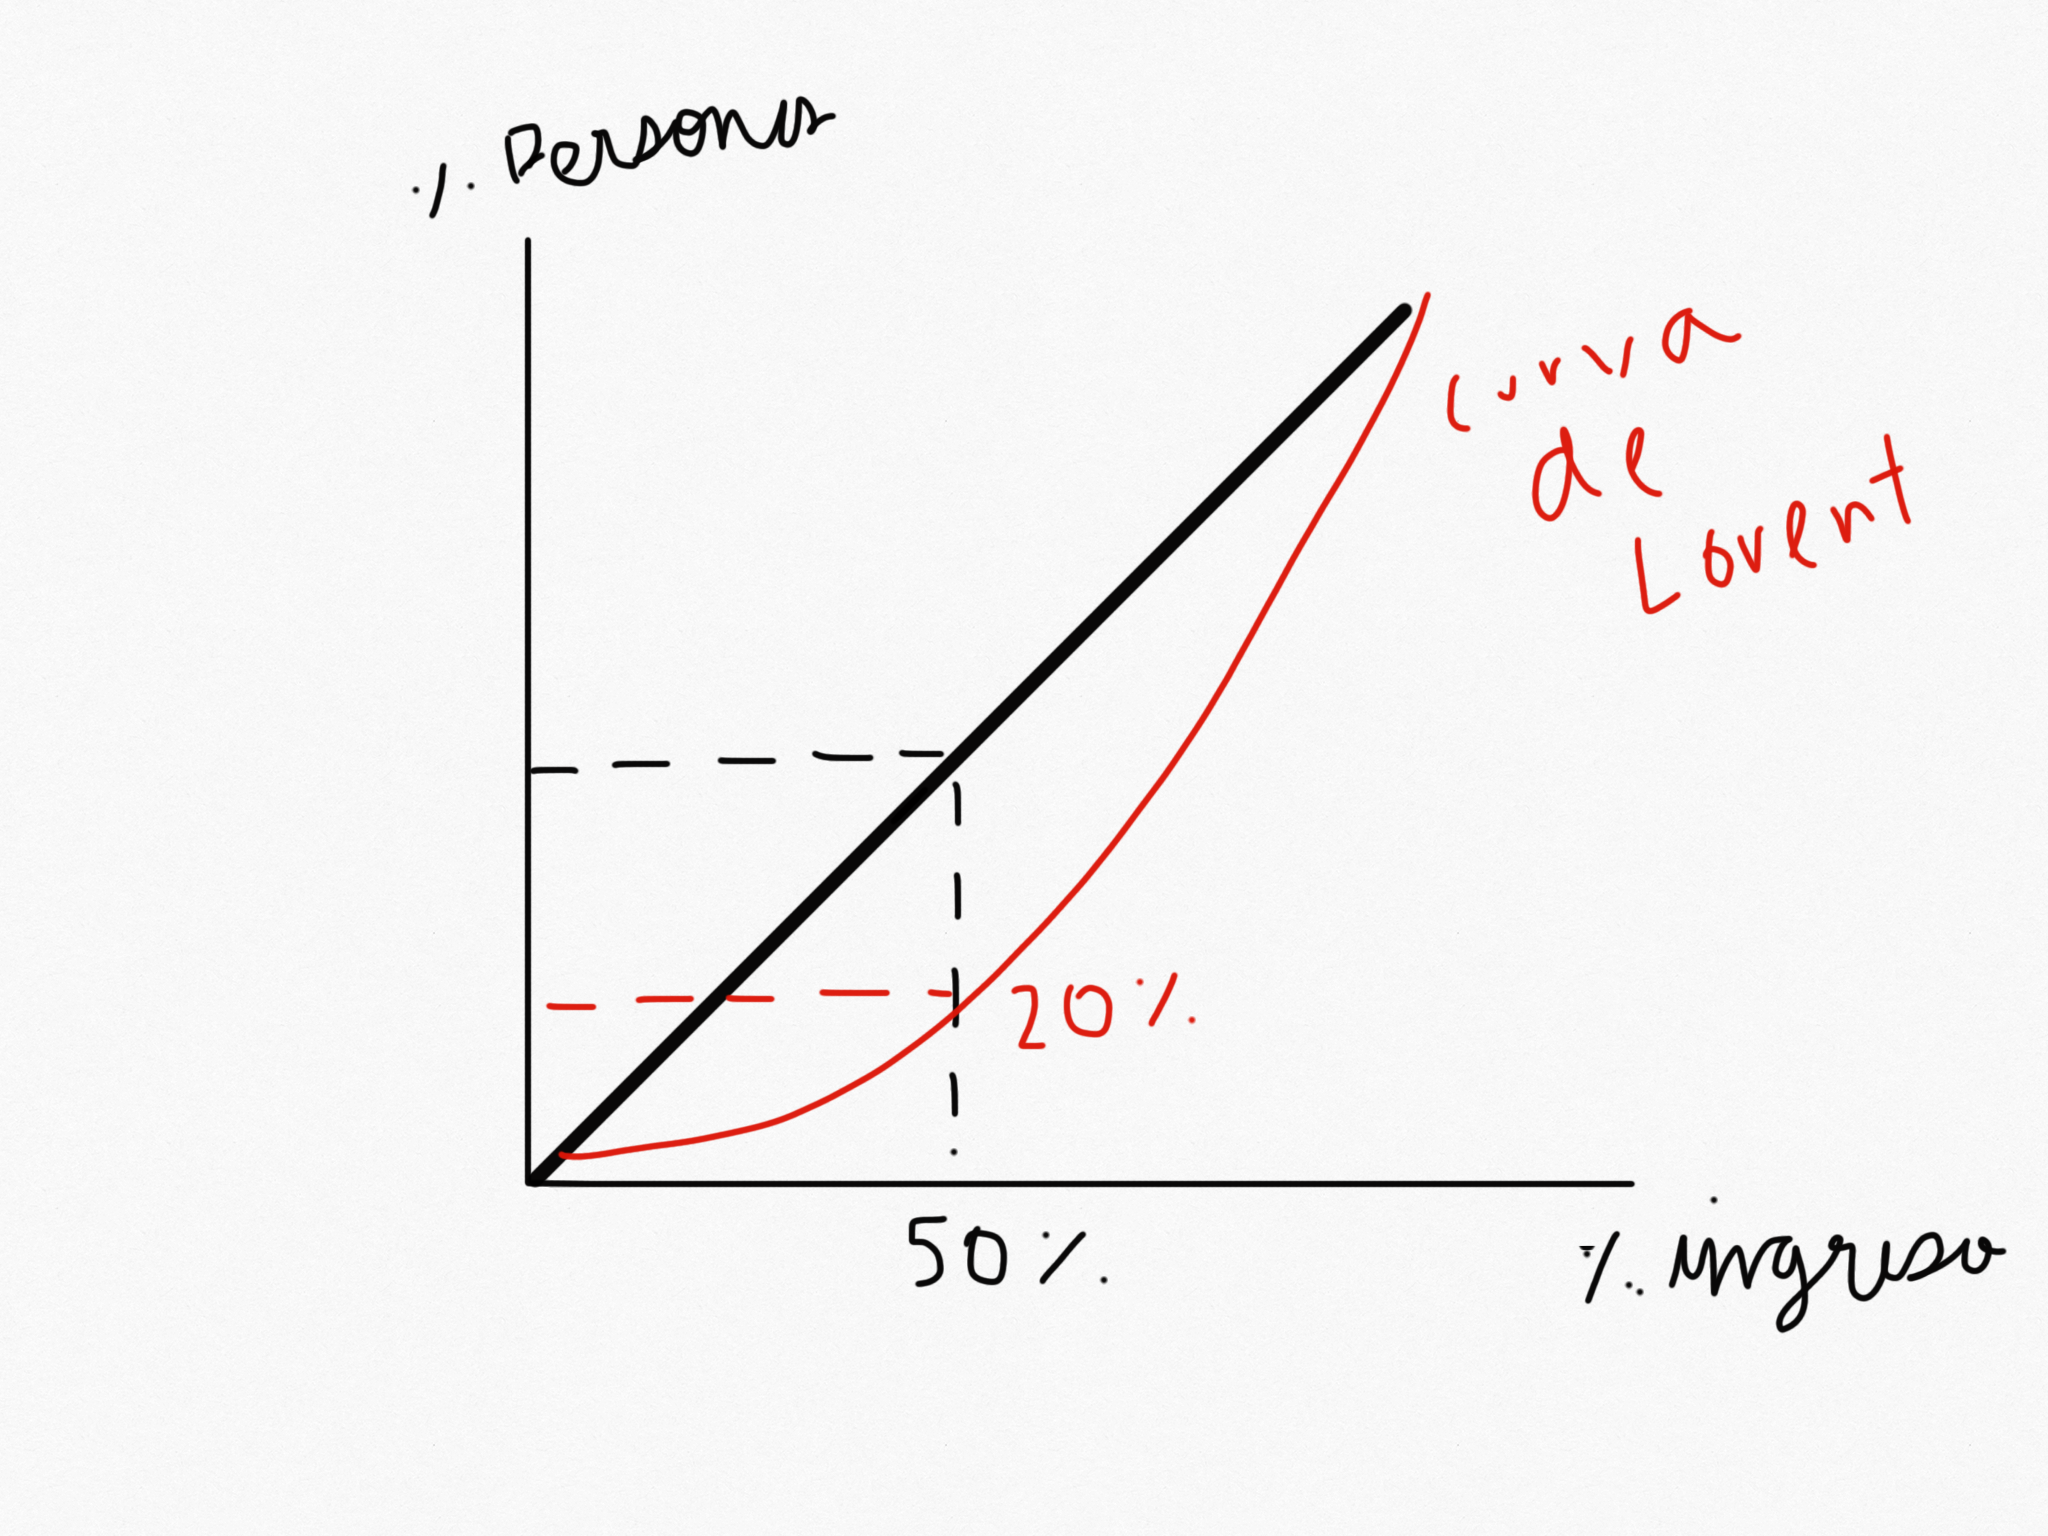
\includegraphics[width=6cm]{Classes/Images/2019-09-16-1.png}
        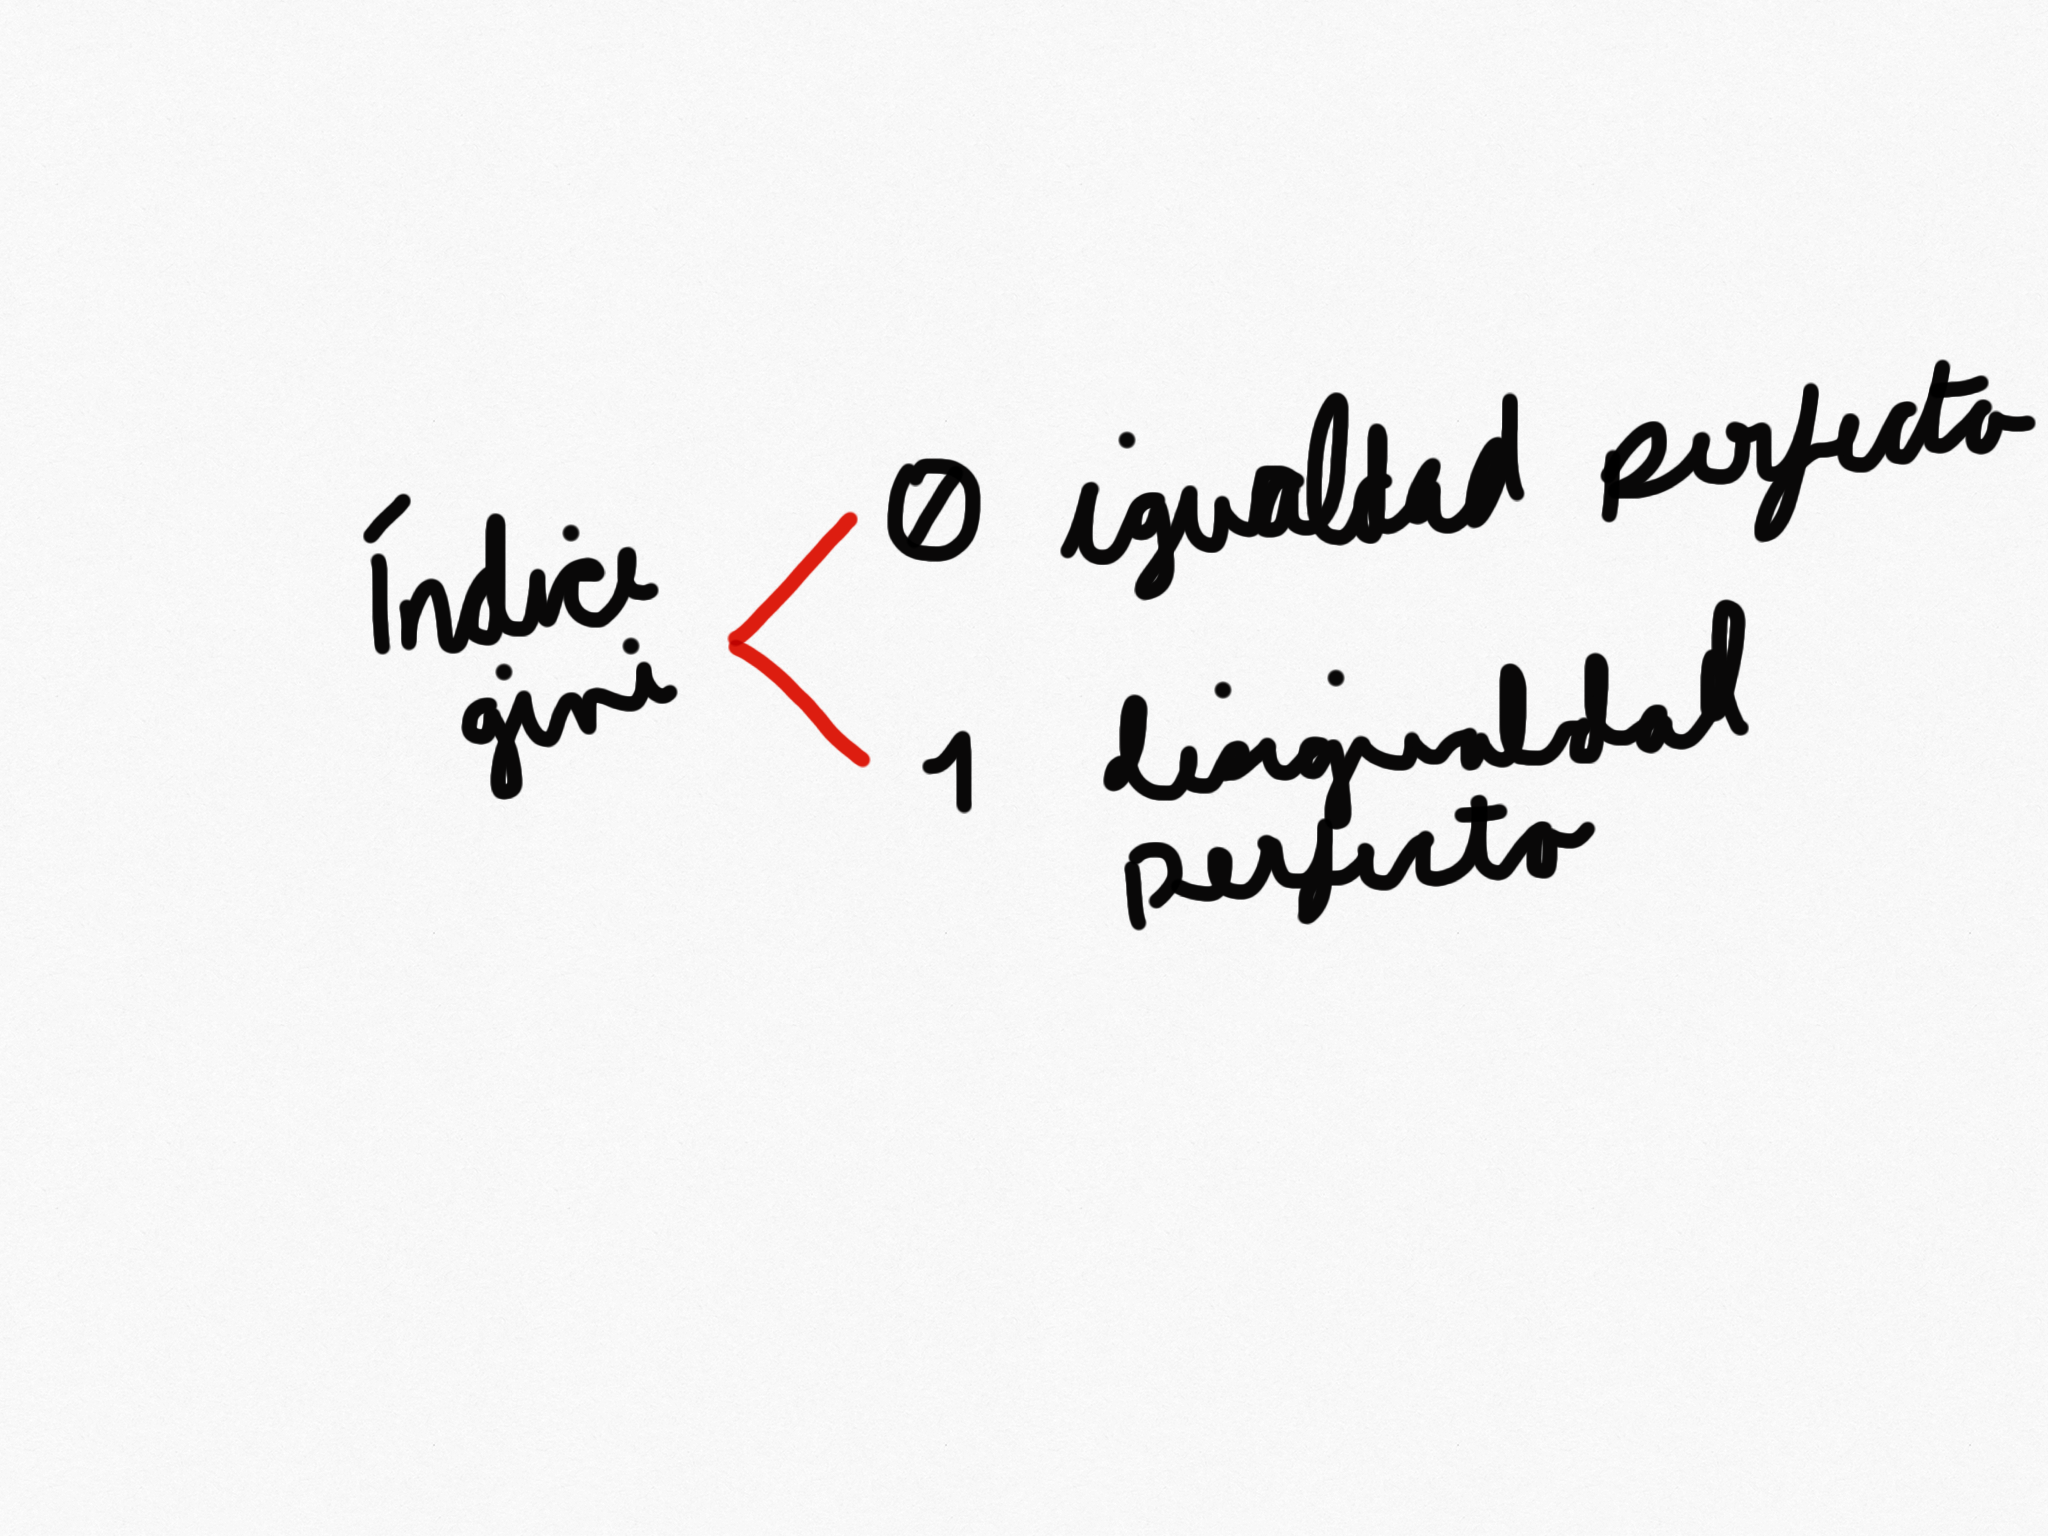
\includegraphics[width=6cm]{Classes/Images/2019-09-16-2.png}
         \caption{}
        \label{}
    \end{figure} 
    
    \item \emph{\textbf{(Paréntesis:}Estimación de la economía de China va a ser más grande que la de EEUU, \textbf{no es cierto que es más rico EEUU que china por la población.} Cuidado con hacer inferencia (la parte más pobre de China != parte más pobre que EEUU)\textbf{)}}.
    \item El PIB puede ser una magnitud flujo y una stock, \emph{\textbf{Ejemplo:} en el horno de pan, el horno es un stock, para el panaero el pan es un flujo} \emph{\textbf{Definición de ``Magnitud de flujo stock":} Flujo: variable cuya cantidad se mide por unidad o periodo determinado de tiempo; por ejemplo, el ingreso, la inversión, el PBI, la inflación, etcétera. Stock: variable cuya cantidad se mide en un determinado momento del tiempo; por ejemplo: la población, la riqueza, el stock de capital, la oferta monetaria, etcétera.}
    \item \emph{\textbf{Observación: }Cuando Daniel se reunió con un funcionario discutiendo discrepancias en las cifras de Ecuador.}
    \item \emph{\textbf{Observación: }Las encuestas de la calidad de vida, el senso, se tardaron una década y no pasó nada.}
    \item El problema de limitar la natalidad es que la taza de natalidad tiene que estar en cierto número entre 20\%$<$natalidad$<70$.
    \item Formas de calcular el PIB: Idealmente las tres fórmulas tienen que coincidir por que los gastos de la gente son ingresos para otra. La diferencia entre el enfoque de gasto (sector formal) y el enfoque de distribución es la informalidad.
    \begin{itemize}
        \item Enfoque del gasto:
        \[
          PIB = C + I_{1} (X -I_{2}) + G 
        \]
        donde C = Consumo, $I_{1}$ = inversión, X = exportaciónes, $I_{2}$ = importaciónes, G = gastos del gobierno \newline 
        En suma, es una forma de medir el PIB por medio del gasto y la inversión de las personas, en cosumo por ejemplo comer, en inversión por ejemplo las inversiones, gastos de gobierno todo los gastos públicos, las remesas son parte del PIB, es la excepción. Se supone que las exportaciones e importaciones son igual a 0 por que las exportaciones tienen que ser financiadas por las importaciones. La informalidad es la diferencia entre los ingresos y los gastos.
        
        \item Enfoque de distribución:
        \[
          PIB = R_{l} + R_{k} + R_{r} +B + A
        \]
        Donde $R_{l}$ es salario, $R_{k}$ es capital, $R_{r}$ es Intereses financieros, B siendo beneficios, A siendo amortizaciónes.
        
        \item Enfoque de producción:
        \[
          PIB = VA_{\text{POR ETAPAS}}
        \]
        Donde VA es valor agregado.
    \end{itemize}
    En economía no se puede calcular objetivamente qué tan preciso es el PIB.
    
    \item PIB vs. Producto Nacional Bruto: 
    \begin{itemize}
        \item PIB: producido interno bruto total de un país.
        \begin{itemize}
            \item El PIB no cubre ni contempla el auto-consumo, esta es la razón por la cual a veces las cifras hace parecer más pobres a los países pobres, economía no monetaria de auto-consumo.
            \item No sale el servicio doméstico.
            \item En EEUU el 75\% del PIB antiguamente era actividades domésticas, por esto es tan caro contratar y la gente entonces deja de producir y hace sus muchas actividades domésticas.
            \item No contempla la prostitución y las drogas así mismo como las actividades monetarias prohíbidas.
            \item En la guerra el PIB sube por agregar a la economía bienes de guerra. \emph{Citación:``Lo mejor para salir de una recesión es una guerra por que sube el PIB"}, esto es falso ya que el PIB sube pero no indica mejor calidad o mejor desarrollo. \emph{Citación: Premio Novel``Que los alienígenas nos invadan y tengamos que desarrollar un programa de defensa"}.
        \end{itemize}
        \item PNB: bienes producidos dentro de la nación. \emph{\textbf{Ejemplo:}de pollo campero en Madrid}.
    \end{itemize}
\end{enumerate}
